\documentclass[../../lecture_notes.tex]{subfiles}

\begin{document}

Let’s look back at our approaches:\\
\indent Imperative — glue together commands via sequencing (side effects are key)\\
\indent Functional — glue together functions (give up side effects)\\
\indent Declarative — glue together predicates with (\&, |, →)\\
\\
It may seem like by using logic programming we are giving up a lot,\\
\indent BUT in return we “don’t have to worry about how our program works”\\
Declarative programs are written by specifying goals rather than methodology\\
In a sense, we declare constraints on a solution, and our interpreter finds a solution.\\
Our algorithms have two major parts:
\begin{enumerate} [itemsep=0mm]
	\item Logic — specifications of correct solutions to the problem
	\item Control — advises the interpreter for efficiency (does not affect speed)
\end{enumerate}
\noindent In a sense, all of our logic programs utilize divide and conquer!\\
The alternative would be Java, which mixes the two parts:\\
	\indent for (i = 0; i < N; i++) f(i); // if we change to i<N-1, it effects correctness.\\
\\
The basics:\\
	\indent pred(Arg1, Arg2, …) forms a goal\\
	\indent ‘,’ is AND \& ‘.’ is end (at the top level)\\
	\indent ‘:-’ is a turnstile that implies “if”\\
	\indent pred(Arg1, Arg2, …) :- cond1, cond2. forms a rule\\
		\indent \indent This means that pred is true if cond1 and cond2 are true\\
\\ 

Our first logic program will be SORTING
\begin{lstlisting} [language=Prolog]
	% First we write specifications for what it means to sort a list
	% L -- unsorted list
	% P -- sorted list
 	% L&P must be permutations of each other
 	% P must be sorted
 	% First we state the top level requirements:
 	sort(L, P) :- permute(L, P), sort(P).
 	% sort is true for L & P if permute and sort are true
 	sorted([]).
 	% the empty list is sorted
 	sorted([_]).
 	% a single element list is sorted
 	sorted([X, [Y|L]) :- X =< Y, sorted([Y|L]).
 	% X::Y::L is sorted if X <= Y and Y::L is sorted
 	permute([], []).
 	% the empty list is a permutation
 	permute([X|L], R) :-
 	permute(L, PL),
 	append(PL1, PL2, PL),
 	append(PL2, [X|PL1], R).
 	append([], L, L).
 	append([X|L1], [X|L2], L) :- append(L1, L2, L).
 	% a fun consequence of this is that we can run code in either direction!
 	?- sort([1, 9, -3], R).
 	R = [-3, 1, 9].
 	?- append([a, b], [c, d, e], R).
 	R = [a, b, c, d, e].
 	?- append(X, [c|Y], [a, b, c, d, e]).
 	X = [a, b].	
 	Y = [d, e].
 	% a predicate can even return multiple; we type ';' to see the next
 	?- append(x, y, [a, b, c, d, e]).
 	x = [], y = [a, b, c, d, e] ;
 	x = [a], y = [b, c, d, e] ;
 	x = [a, b], y = [c, d, e] ;
 	x = [a, b, c], y = [d, e] ;
 	x = [a, b, c, d], y = [e] ;
 	x = [a, b, c, d, e], y = [] ;
 	no.
\end{lstlisting}

\noindent This should have been obvious to us; we utilize append in this way in our code!\\
While our code is simple and documents itself well, append is O(N), so permute and sort are O(N!)\\
This may lead one to think Prolog is inefficient, but consider the N-Queens problem;
\indent Prolog can solve it in 3 lines of code at roughly C speed!\\
It is up to us to utilize Prolog in an efficient way!
\\
We will now lay out the basic syntax of Prolog (Edinburgh Syntax):
A Prolog term is one of:
\begin{enumerate} [itemsep=0mm]
	\item atom — ${\#, [a-z][A-Za-z\_0-9]*}$\\
		These represent constants within our programs.\\
		Alternatively, we can use single quotes to turn anything into an atom.\\
		Atoms are unique and equivalent to only themselve.\\
	\item (logical) variable — $[\_A-Z][A-Za-z\_0-9]*$\\
		Variables are bound/instantiated on success.
		They are only unbound on failure.
		Bound variable assignments cannot be changed
		We avoid names beginning with ‘\_’; these are generated by the interpreter
	\item structure — {atom(term1{, term}*)}\\
		The starting atom is called the functor.\\
		We refer to a structure by functor/\#args\\
		The name is apropos; these are represented as trees
\end{enumerate}
\begin{center} \begin{tikzpicture}
	\node (1) {f(g(x), h(i(27))};
	\node [rectangle, draw, align=center, below =of 1] (2) {\begin{tabular} { c | c | c} f & . & . \end{tabular}};
	\node [rectangle, draw, align=center, below =of 2] (3) {\begin{tabular} { c | c} g & x \end{tabular}};
	\node [rectangle, draw, align=center, below right =of 3] (4) {\begin{tabular}{ c | c} h & . \end{tabular}};
	\node [rectangle, draw, align=center, below right =of 4] (5) {\begin{tabular}{ c | c} i & 27 \end{tabular}};
	\draw[->] (1.south) -- (2.north west);
	\draw[->] (2.south) -- (3.north west);
	\draw[->] (2.south east) -- (4.north west);
	\draw[->] (4.south east) -- (5.north west);
\end{tikzpicture} \end{center} \medskip

\noindent That’s it! Anything else we have seen is only “syntactic sugar”
\begin{itemize} [itemsep=0mm]
	\item $[]$ == ‘[]’
	\item $[a, b, c]$ == ‘.’(a, ‘.’(b, ‘.’(c, ‘[]’)))
 	\item $[X, Y|Z]$ == ‘.’(X, ‘.’(Y, Z))
 	\item a :- b, c, d. == ‘:-’(a, ‘,’(b, ‘,’ (c, d)))
\end{itemize}
\noindent But if predicates are represented as structures, how do we actually evaluate them?\\
\indent We use the keyword ‘is’
\begin{lstlisting} [language=Prolog]
	?- N is 2+2.
	N = 4.
	?- is(N, 2+2).
	N = 4.
\end{lstlisting}
\noindent This tends not to be used much, since declarative statements are rare in Prolog.\\
Prolog instead tends to represent first-order logic\\
\\
Structures can take one of three forms:
\begin{enumerate}
\item fact — a statement that is true
\begin{lstlisting} [language=Prolog]
	true.
	prereq(CS31, CS131).
	prereq(CS31, CS111).
	equals(X, X).
\end{lstlisting}
\item rules — a predicate that is conditionally true
\begin{lstlisting} [language=Prolog]
	ipr(A, B) :- prereq(A, Q), ipr(X, B).
	ipr(A, B) :- prereq(A, B).
 	% this compiles fine, but the below causes an infinite loop:
 	ipr(A, B) :- prereq(A, B).
 	ipr(A, B) :- prereq(A, Q), ipr(X, B).
 	% all of these rules are considered the same predicate, 
 	% since they share functor and argument count
 	c. goals - queries to be evaluated
 	?- X = 3.
 	X = 3.
 	yes.
 	?- ipr(CS31, Z).
 	Z = CS131? ;
 	Z = CS111? ;
 	no.
\end{lstlisting} \medskip
\end{enumerate}
\subsubsection*{Failure}
\noindent In the real world, we have TRUE, FALSE, and UNKNOWN, BUT\\
	\indent in C/Java we have T or F and we deal with unknowns.\\
	\indent in Prolog we have success or failure to prove.\\
Thus failure becomes a major factor in flow control.\\
\\
A simple example:
\indent Say the registrar provides us with the following predicate:
\begin{lstlisting} [language=Prolog]
	prereq(CS31, CS32).
 	prereq(CS31, CS111).
 	prereq(CS31, CS131).
 	prereq(CS131, CS132).
\end{lstlisting}
Can we conclude that dance 101 is not a prerequisite for CS131?\\
	\indent Logically NO, we just can’t prove it,\\
	\indent BUT in prolog we assume a closed world and thus that the list is complete\\
	\indent Therefore, this would fail!

\subsubsection*{Ordering}
\noindent A clause can refer to a predicate not yet defined so long as it is defined at usage time.
While ordering does not affect correctness (in general), it affects efficiency.\\
\\
Prolog is goal oriented, so the search is bottom up.\\
We backward-chain to build a search tree\\
	\indent leaves = facts\\
	\indent branches = successful rules\\
Failed rules are removed from the tree\\
A parse tree is a form of search tree — it proves a sentence validity in a grammar.\\

At any point in time, Prolog has a partially build tree.\\
It matches the provided goal to the heads of the clauses, in order, until it finds a match, when:
\begin{enumerate} [itemsep=0mm]
	\item it is a fact => we have a leaf
	\item it is a rule => we have a subgoal to evaluate!
\end{enumerate}
The interpreter then works on subtrees from left to right, depth-first, and backtracking.\\

\begin{center} \begin{tikzpicture}
	\node[ellipse, draw] (1) {Goal};
	\node[ellipse, draw, below left =of 1] (2) {I};
	\node[rectangle, draw, below =of 2] (3) {fact};
	\node[ellipse, draw, below right =of 1] (4) {J};
	\draw [->] (1.south) -- (2.north);
	\draw [->] (2.south) -- (3.north);
	\draw [->] (1.south) -- (4.north);
	\node[right =of 4, text width=4.5cm] {\parindent=2em
							ipr(A,B) = \\ 
							\indent match G to \\ 
							\indent \indent H := I, J\\
							\indent \indent \indent H = ipr(X, Y)\\
							\indent \indent \indent J = prereq(X, M)\\
							\indent \indent \indent I = ipr(M, Y)};
\end{tikzpicture} \end{center}

Infinite loops are relatively easy to fall into:
\begin{lstlisting} [language=Prolog]
	memb(X, [X|_]).
 	memb(X, [_, L]) :- memb(X, L).
 	/* the standard forward usage would be: */
 	|?- memb(X, [a, b, c, d, e]).
	X = a? ;
	X = b? ;
	X = c? ;
	X = d? ;
	no.
	/* we can get strange repeat cases:*/
	|?- memb(a, [a, b, x, y, d, e, z]).
	true? ;
	X=a? ;
	Y = a? ;
	Z = a? ;
	no.
	/* we can even test the goal without any literals */
	|?- memb(A, B).
	B = [A|_]? ;
	B = [_, A|_]? ;
	B = [_, _, A|_]? % this gives us an infinite loop!
	app([], L, L).
	app([X|L], M, [A|LM]) :- app(L, M, LM).
	|?- app(X, Y, [a, b, c]).
	X = []
	Y = [a, b, c]? ;
	X = [a]
	Y = [b, c]? ;
	X = [a, b]
	Y = [c]? ;
	X = [a, b, c]
	Y = []? ;
	no.
	/* even this predicate is not safe, though: */
\end{lstlisting}
\noindent We will now write our canonical reverse:
\begin{lstlisting} [language=Prolog]
 	naive_reverse([], []).
 	naive_reverse([X|Y], Rx) :- naive_reverse(L, R), append(R, [x], Rx).
 	% this is O(N^2); we must use a general solution with an accumulator!
 	revapp([], A, A).
 	revapp([X|L], A, R) :- revapp(L, [X|A], R).
 	% now for the application:
 	fast_reverse(L, R) :- revapp(L, [], R).
 	% We can compare the two implementations:
 	|?- naive_reverse([a, b, c], R).
 	R = [c, b, a].
 	|?- fast_reverse([a, b, c, d, e, f, g], R).
 	R = [g, f, e, d, c, b, a].
 	|?- naive_reverse(L, [a, b, c, d]).
 	L = [d, c, b, a]? ;
 	Fatal Error: global stack overflow!
 	% what happened? can fast_reverse handle it?
 	|?- fast_reverse(L, [a, b, c, d]).
 	L = [d, c, b, a]? ;
 	Fatal Error: global stack overflow!
\end{lstlisting}
\newpage
How can we debug this?\\
\indent We use the Four Port Debug Model
\begin{figure}[H]
	\centering
	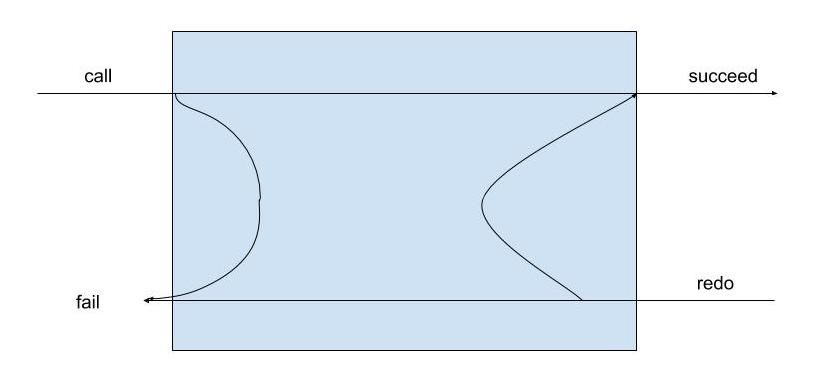
\includegraphics[width=\textwidth]{debug_model}
	\caption{We place a "spy" at each port}
	\label{fig:test}
\end{figure}

\begin{lstlisting} [language=Prolog]
 	| ?- trace, naive_reverse(L, [a,b]).
 	The debugger will first creep -- showing everything (trace)
 	1 1 Call: naive_reverse(_23,[a,b]) ?
 	2 2 Call: naive_reverse(_63,_102) ?
 	2 2 Exit: naive_reverse([],[]) ?
 	3 2 Call: append([],[_62],[a,b]) ?
 	3 2 Fail: append([],[_62],[a,b]) ?
 	2 2 Redo: naive_reverse([],[]) ?
 	3 3 Call: naive_reverse(_89,_128) ?
 	3 3 Exit: naive_reverse([],[]) ?
 	4 3 Call: append([],[_88],_156) ?
 	4 3 Exit: append([],[_88],[_88]) ?
 	2 2 Exit: naive_reverse([_88],[_88]) ?
 	5 2 Call: append([_88],[_62],[a,b]) ?
 	5 2 Exit: append([a],[b],[a,b]) ?
 	1 1 Exit: naive_reverse([b,a],[a,b]) ?
 
 	L = [b,a] ? ;
 	1 1 Redo: naive_reverse([b,a],[a,b]) ?
 	2 2 Redo: naive_reverse([_88],[_88]) ?
 	3 3 Redo: naive_reverse([],[]) ?
 	4 4 Call: naive_reverse(_115,_154) ?
 	4 4 Exit: naive_reverse([],[]) ?
 	5 4 Call: append([],[_114],_182) ?
 	% the system finds a match of the appropriate length, 
 	% and if we continue it looks for a longer one, which it won't find!
 	% NOTE: we could also perform a manual debug if we wanted ("app" is self-chosen)
 	|?- append(X, Y, [a, b, c, d]), write(app(X, Y)), nl, fail.
\end{lstlisting}

\subsubsection*{Unification}
$\equiv$ the process of making two terms equal\\
Consider: f(g(Y), h(Z)) - f(A, h(i(B))) $\rightarrow$ f(g(Y), h(Z))\\
	\indent {A = g(Y), z = i(B)} is called the unifier, and it makes the statements equivalent.\\
When we have earlier said "matching" heads, we were referring to unifying.\\
We use the following terminology:\\
	\indent Fact: p(a, b)\\
	\indent Goal: p(X, b)\\
	\indent Unifier: {X=a}\\
This is used to transmit information from the callee to the caller.\\
\\
Matching can even bind variables:\\
	\indent Fact: p(X, b) :- q(X)\\
	\indent Goal: p(a, b)\\
Thus we can see that unifying is more powerful than matching or switches;\\
	\indent these let us take apart values, but Prolog can let you build as well!
\\
A single unification can even communicate in both directions!\\

\begin{center} \begin{tikzpicture}
	\node[text width=5cm] (text) {Fact: e(X, X) \\ Goal: e(Y, f(y)) \\ |?- e(Y, f(Y)). \\ $\rightarrow$ Y=f(f(...};
	\node[rectangle, draw, right =of text] (l) {Y};
	\node[rectangle, draw, right =of l] (r) {\begin{tabular} { c | c } f & . \end{tabular}};
	\draw[->] (r.south east) to [out=210, in=330] (l.south);
	\draw[->] (l.north) to [out=30, in=150] (r.north west);
\end{tikzpicture} \end{center}		

\indent Fact: f(g(Y), h(Z))\\
\indent Goal: f(A, h(i(B)))\\
BUT this can lead us into trouble...
\begin{enumerate} [itemsep=0mm]
	\item we could get an infinite loop ->
	\item we could break the logic of a problem!
\end{enumerate}
\noindent Consider the example of Peano Arithmetic:\\
	\indent We wish to come up with a logical basis for mathematics.\\
	\indent Peano decided to implement nonnegative integer arithmetic.
	\indent But Godel's Incompleteness Theorem says a logic cannot prove itself!\\
 Let's try anyway:
 \begin{lstlisting} [language=Prolog]
	% zero = 'zero'
	% N+1 = 'succ(N)'
	sum(zero, N, N).
 	sum(succ(N), M, succ(NplusM)) :- sum(N,M,NplusM).
\end{lstlisting}

\subsubsection*{Control}
\noindent We can actually model our tree a different way:\\
	\indent leaves are answers\\
	\indent nodes are “choice points”\\
In this model, our behavior at choice points determines our efficiency; this is called \textbf{\underline{control}}.\\
Consider the following examples:
\begin{lstlisting} [language=Prolog]
	fail. % this is hard wired, and produces an empty search tree
 	true. % this forms a tree with a single node
 	% the following is akin to C's while(true), and is built in
 	repeat.
 	repeat :- repeat.
 	|?- repeat, write(X), fail. % infinite loop of X's
 	% this forms a right-recursive search tree, and finds infinite solutions
 	% the following is not built in, but is logically equivalent to repeat
 	loop :- loop.
 	loop.
 	% this forms a left recursive search tree, and thus will find no solution!
 	% it therefore cannot be proven
\end{lstlisting}
\noindent Suppose we have the following search tree:

\begin{center} \begin{tikzpicture}
	\node (tree) {a}
		child {node {b}
			child {node {c}
				edge from parent {}
			}
			child {node {d}
				edge from parent {}
			}
			child [missing]
			edge from parent {}
		}
		child {node {e}
			child[missing]
			child{node {f}
				child{node {g}
					edge from parent {}
				}
				child{node {h}
					child{node{i}
						child  {node {k}
							edge from parent {}
						}
						child {node {l}
							edge from parent {}
						}
						edge from parent {}
					}
					child{node{j}
						edge from parent {}
					}
					edge from parent {}
				}
			edge from parent{}
			}
			child {node {m}
				edge from parent{}
			}
			edge from parent {}
		};
	\node[text width=10cm, below right =4cm of tree] {
								Suppose we are at point g.\\
								Suppose we know that if we fail, the sibling subtree of h will.\\
								Then we can use the cut (!) to  prune alternatives.\\
								The cut succeeds on first encounter,  but fails on backtrack.\\
								Doing this increases the efficiency of our programs!};
\end{tikzpicture} \end{center} 

The usage is as follows:
\begin{lstlisting} [language=Prolog]
 	complicated(X, Y, Z) :- generate(X, Y, Z), test(X, Y, Z).
 	% suppose we know that test/3 is slow and will fail unless X is in Y
 	% we can thus perform this check before performing our slow function
 	complicated(X, Y, Z) :- generate(X, Y, Z), member(X, Y), test(X, Y, Z).
 	% this still has an efficiency problem! 
	% consider X = a, Y = [a, b, c, a, c, a, d, a]
 	% our program will perform test 4x more than necessary!
 	% we can improve this with the cut!
 	memberchk(X, [X|_]) :- !.
 	memberchk(X, [_|L]) :- memberchk(X, L).
 	% thus we can greatly improve our efficiency:
 	complicated(X, Y, Z) :- generate(X, Y, Z), memberchk(X, Y), test(X, Y, Z).
\end{lstlisting}
\noindent This is great, but the cut is very much the ‘goto’ of prolog: it is risky!
\begin{lstlisting} [language=Prolog]
 	\+(P) :- P, !, fail.
 	\+(_).
 	% this only succeeds if P is false! 
 	% it is not equivalent to 'not', consider:
 	|?- X=1, \+(X=2), write(ok).
 	% writes 'ok'
 	|?- \+(X=2), X=1, write(ok).
 	% fails, since X is already bound to 1
 	% thus \+ is not commutative!
\end{lstlisting}
\noindent This may seem like semantic nitpicking, but the idea is actually central to prolog.\\
For example, theoreticians would say \\
	\indent $\vdash$P means “P is provable”\\
 	\indent $\models$P means “P is true”\\
These may seem equivalent, but they very much are not!\\
	\indent  $\vdash$P but not $\models$P $\implies$ your logic is inconsistent (BAD)\\
 	\indent $\models$P but not $\vdash$P $\implies$ your logic is incomplete (DISAPPOINTING)\\
The goal of developing a logic is to meet both requirements\\
This has been met for some subsets of logic (Euclidian Geometry, etc.).\\
This is not possible for integer arithmetic due to Godel’s Theorem/Turing’s Halting Problem\\
\\
Thus $\backslash$+ really means “not provable” (It even looks like $\not\models$)\\
The closed world assumption lets us use $\backslash$+ in some cases:
\begin{lstlisting} [language=Prolog]
 	prereq(CS31, CS131).
 	% ...
 	|?- \+ prereq(dance101, CS131).
 	% succeeds, which is correct with a closed world
 	|?- \+(X=1).
 	% fails, since X is not currently bound
 	% we thus call X a ground term, 
	% and we insist \+ takes only ground terms
\end{lstlisting}
\end{document}